\documentclass{article}
\usepackage{fontspec}

% Used to embed Sage code in latex
%\usepackage{sagetex}


% Math Environment
\usepackage{euler}        % Euler font
\usepackage{amsmath}      % Math macros
\usepackage{amssymb}      % Math symbols
\usepackage{unicode-math} % Unicode support

% Physics Environment
\usepackage{physics}


\usepackage[makeroom]{cancel} % Used to cancel terms in algebraic equations
\usepackage{ulem} % Different underline environments
\usepackage{polynom} %Polynomial long division

% Typesetting Rules
\setlength\parindent{0em}
\setlength\parskip{0.618em}
\usepackage[a4paper,lmargin=1in,rmargin=1in,tmargin=1in,bmargin=1in]{geometry}
\setmainfont[Mapping=tex-text]{Helvetica Neue LT Std 45 Light}

% Common Macros
\newcommand\N{\mathbb{N}}
\newcommand\Z{\mathbb{Z}}
\newcommand\Q{\mathbb{Q}}
\newcommand\R{\mathbb{R}}
\newcommand\C{\mathbb{C}}
\newcommand\A{\mathbb{A}}
\def\res{\mathop{\text{Res}}\limits}

% Color
\usepackage[dvipsnames]{xcolor}
\usepackage{pagecolor}
% \definecolor{DeepMossGreen}{HTML}{394820}
% \pagecolor{DeepMossGreen}
% \color{Goldenrod}

\usepackage{graphicx}

\begin{document}

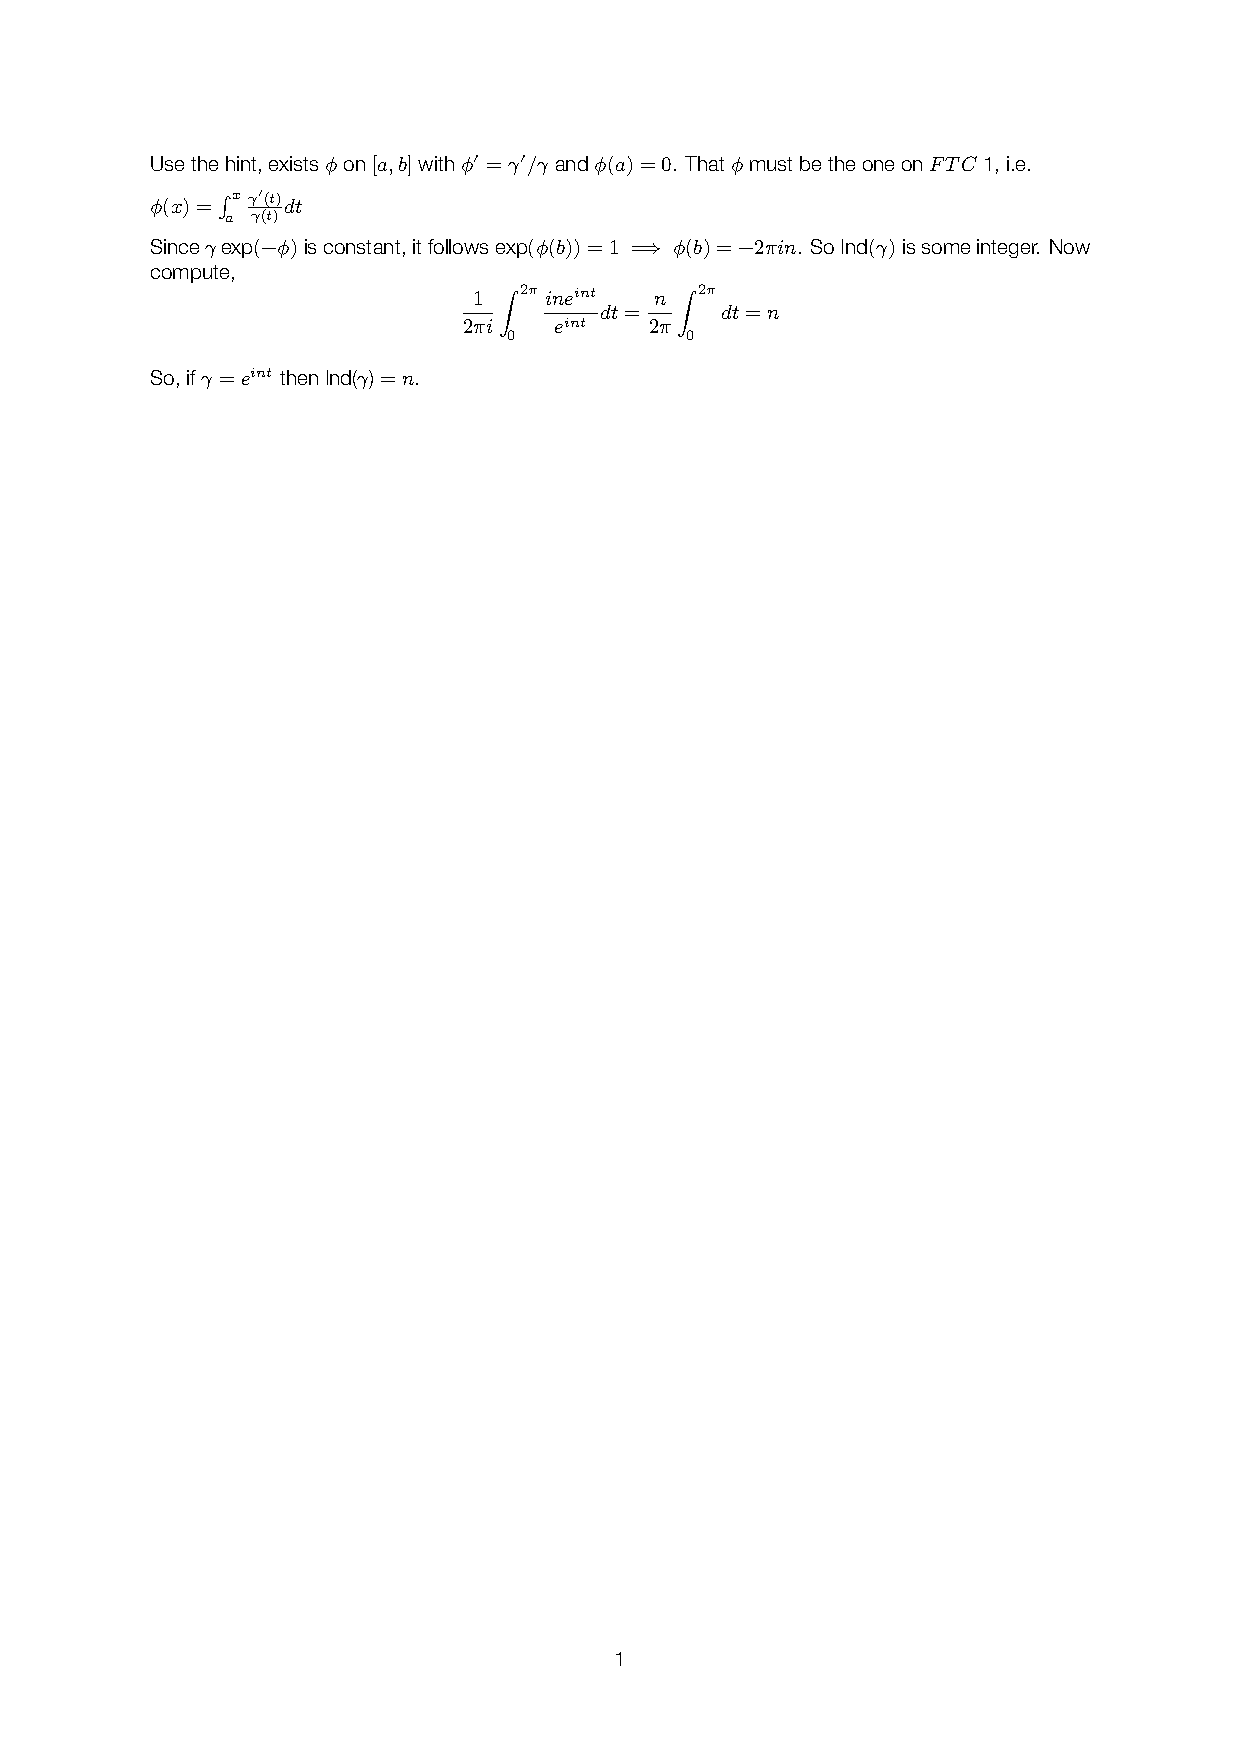
\includegraphics[width=\textwidth]{q3.png}

\uwave{pf.}

(a) By the AM-GM inequality,
\[x^4>0, y^2 >0 \implies \sqrt{x^4y^2} \leq \frac{x^4+y^2}{2}
  \implies 4x^4y^2 \leq ({x^4+y^2})^{2}.\]

$f$ is differentiable, for $(x,y)\neq (0,0)$, so it's enough to show
$f$ is continuous at $(0,0)$
\[|f(x,y)| = |x^2+y^2 -2x^2y - \frac{4x^6y^2}{({x^4+y^2})^{2}}| <
  |x^2+y^2| +2x^2|y| +x^2\bigg|\frac{4x^4y^2}{({x^4+y^2})^{2}}\bigg|\]

From the first inequality we have,
\[4x^4y^2 \leq ({x^4+y^2})^{2} \implies 0 \geq
  \frac{4x^4y^2}{({x^4+y^2})^{2}} \leq 1 \implies 0 \geq x^2
  \frac{4x^4y^2}{({x^4+y^2})^{2}} \leq x^2\]

So as $x\rightarrow 0$, $\frac{4x^6y^2}{({x^4+y^2})^{2}} \rightarrow
0$. So as $(x,y)\rightarrow 0$, $f(x,y)\rightarrow 0$. Therefore, $f$
is continuous.

(b) Plugging in,
\[g_\theta(t) =  t^2 -2t^3\cos^2(\theta)\sin(\theta)
  -\frac{4t^4\cos^6(\theta)\sin^2(\theta)}{(t^2\cos^4(\theta)+\sin^2(\theta))^2}\]

If $\theta =  0$, $g_0(t) = t^2\implies g_0(0) = 0,g^\prime_0(0) = 0,$
and $g^{\prime\prime}_{0}(0) = 2$. We need to consider it separately
because if $\theta =  0 = t$, then
$(t^2\cos^4(\theta)+\sin^2(\theta))^2 = 0$.

Now, for $\theta \neq 0$, plugging in $0$,
\[g_\theta(0) =  0\]

Differentiating with respect to $t$,
\[g^{\prime}_\theta(t) =  2t -6t^2\cos^2(\theta)\sin(\theta)
  -\frac{16t^3\cos^6(\theta)\sin^2(\theta)}{(t^2\cos^4(\theta)+\sin^2(\theta))^2}\]

Plugging in $0$,
\[g_\theta^\prime(0) =  0\]

Differentiating with respect to $t$,
\[g_\theta^{\prime\prime}(t) =  2 -12t\cos^2(\theta)\sin(\theta)
  -\frac{48t^2\cos^6(\theta)\sin^2(\theta)}{(t^2\cos^4(\theta)+\sin^2(\theta))^2}\]

Plugging in $0$,
\[g_\theta^{\prime\prime}(0) =  2\]

So each $g_\theta$ has a strict local minimum at $t=0$.

So the restriction of $f$ to each line through $(0,0)$, has a strict
local minimum at $(0,0)$.

(c)
Computation shows,
\[f(x,x^2) = x^2 +x^4-2x^4 -x^2 = -x^4\]

Let $\varepsilon > 0 $. Since, \[f(0,0) = 0 > -\varepsilon^4 =
  f(\varepsilon,\varepsilon^2)\]
$(0,0)$ can't be a local minimum of $f\quad \blacksquare$
\end{document}



%%% Local Variables:
%%% mode: latex
%%% TeX-master: t
%%% End:
